\chapter{Introducción}

Durante décadas, el mundo del videojuego se ha ido abriendo paso como uno de los principales entretenimientos de la sociedad. Ya desde su nacimiento, 
no ha sido considerado barato, y todavía sigue con esa tendencia aunque cada vez sea más fácil encontrar ciertos títulos a menor precio.

Es por eso que se intenta encontrar ofertas en las tiendas, tanto las especializadas en videojuegos como las grandes superficies, para poder comprar 
los juegos a un precio más bajo, ya sea por seguir un presupuesto marcado, por optar a comprar más de un título o más razones que se pueden llegar a 
dar.

También la demografía de los jugadores ha ido cambiando con el paso del tiempo. En un principio, los videojuegos eran un entretenimiento para niños, pero 
ahora contamos con una gran cantidad de jugadores que sobrepasan los 25 años de edad según los datos que la Asociación Española de Videojuegos\cite{aevi} 
dio el año pasado.

Es por eso que, teniendo en cuenta que el público mayoritario es un público adulto, se han llegado a crear plataformas donde llegar a compartir las 
distintas ofertas que los usuarios han ido encontrando. Estas plataformas se pueden encontrar en distintos formatos, aunque principalmente se suele 
utilizar Telegram\footnote{Más información de la aplicación en su página web: https://telegram.org/} o Discord\footnote{Puede encontrarse más información 
en la página https://discord.com/} por sus opciones de canales\footnote{Más información sobre los canales de Telegram en 
https://telegram.org/tour/channels/es?ln=a} y servidores\footnote{Más información sobre los servidores de Discord en https://discord.com/servers} 
respectivamente.

Un ejemplo de esto es el canal Ofertas Juegos en Telegram\footnote{Tienen su propia página web (https://ofertasjuegos.es/) con toda la información} 
(fig. \ref{fig:canal_telegram_ofertas}). Este canal añade un mensaje por cada nueva bajada de precio de cualquier producto en cada tienda, siendo 
diferentes usuarios los que aportan estas ofertas mientras van buscando el mejor precio para el videojuego que quieren comprar.

\begin{figure}[h]
    \centering
    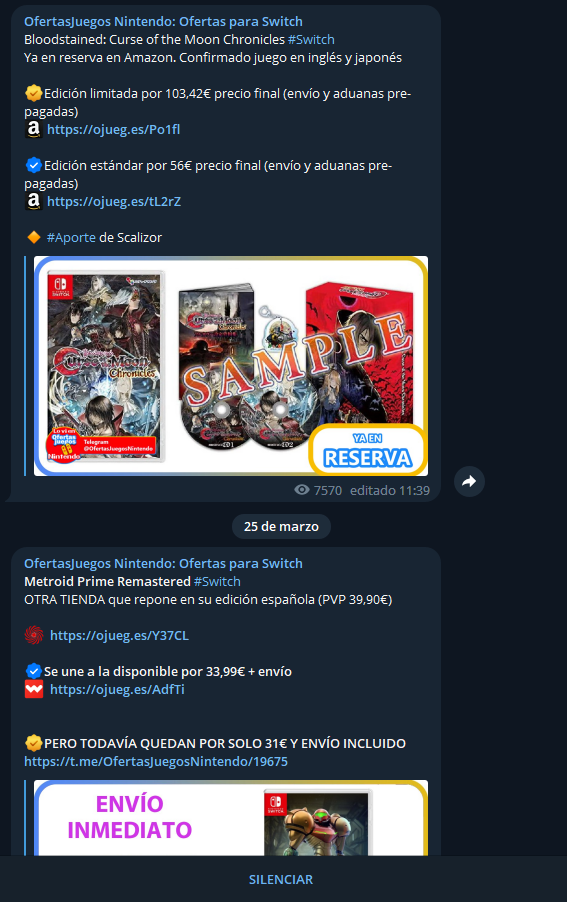
\includegraphics[scale=0.57]{figuras/canal_telegram_ofertas}
    \caption{Ejemplo de canal de ofertas en Telegram.}
    \label{fig:canal_telegram_ofertas}
\end{figure}

De por sí, esto parece más que una solución viable para la mayoría de la gente, pero encontramos un problema: \textbf{si se quiere comprar un videojuego en 
concreto, puede llegar a ser bastante difícil encontrar la última oferta del producto que queramos adquirir por cada una de las tiendas si se han dado 
otras ofertas para otros productos.}

Contando con esto, podemos decir que el objetivo de este proyecto es el siguiente:

\begin{enumerate}
    \item{Construir un bot para Telegram que permita obtener la última oferta de cada tienda para el título por el que se le pregunte.}
    \item{Construir un bot para Discord que ofrezca el mismo servicio.}
    \item{Se publicarán para su uso en sus respectivas plataformas.}
\end{enumerate}
